\documentclass[conference]{IEEEtran}
\IEEEoverridecommandlockouts

\usepackage{cite}
\usepackage{amsmath,amssymb,amsfonts}
\usepackage{algorithmic}
\usepackage{graphicx}
\usepackage{textcomp}
\usepackage{xcolor}
\usepackage{booktabs}
\usepackage{multirow}
\usepackage{array}

\graphicspath{{../results/}}

\begin{document}

\title{Permutation-Invariant Deep Reinforcement Learning for Cross-Trace Cloud Load Balancing}

\author{
\IEEEauthorblockN{Ambika Prasad Rath}
\IEEEauthorblockA{\textit{Department of Computer Science} \\
\textit{NIST University}\\
India}
\and
\IEEEauthorblockN{Prof. Sobhana Behera}
\IEEEauthorblockA{\textit{Department of Computer Science} \\
\textit{NIST University}\\
India}
}

\maketitle

\begin{abstract}
Cloud load balancing must adapt to dynamic workload patterns without manual reconfiguration. Reinforcement learning (RL) offers a promising alternative to static heuristics, but existing RL approaches rely on fixed-architecture deep Q-networks that struggle to represent permutation-invariant routing policies across unordered virtual machines (VMs). This paper presents a permutation-invariant DQN architecture that treats VMs as interchangeable entities, enabling competitive performance against hand-crafted heuristics. We train on the Google Borg 2019 trace and evaluate zero-shot on the Alibaba 2018 container trace. Our results demonstrate three findings: (i) a pointer-style network achieves -0.340 reward on Google, matching the Greedy-Load heuristic (-0.328) and significantly outperforming an MLP baseline (-0.598); (ii) the trained policy exhibits asymmetric transfer, improving load imbalance by 71.6\% on the unseen Alibaba trace while degrading response time by 165.8\%; and (iii) the transferred policy outperforms Greedy-Load on Alibaba by 0.009 reward units, demonstrating that learned representations transfer better than hand-crafted rules under distribution shift. All differences are statistically significant at $p < 0.001$.
\end{abstract}

\begin{IEEEkeywords}
Cloud computing, load balancing, reinforcement learning, deep Q-network, permutation-invariant, cross-trace generalization
\end{IEEEkeywords}

% ============================================================
\section{Introduction}
% ============================================================

Cloud computing has become the dominant paradigm for delivering computing resources over the internet, with major providers including Amazon Web Services, Microsoft Azure, and Google Cloud Platform serving millions of customers worldwide. As cloud adoption grows, efficiently distributing incoming requests across heterogeneous virtual machines (VMs) has become a critical challenge. An effective load balancer must ensure that no single VM becomes overwhelmed while others remain idle, thereby maximizing throughput and minimizing response time.

Traditional load balancing algorithms fall into three categories. Static algorithms such as Round Robin (RR) cycle through VMs in fixed order, ignoring actual load. Dynamic algorithms such as Least Connections (LC) and Throttled (TH) consider current system state but rely on heuristics. Adaptive algorithms attempt to learn from observed outcomes but typically require manual tuning. None of these approaches can dynamically discover optimal routing policies from experience.

Reinforcement learning (RL) offers a natural framework for adaptive load balancing: an agent interacts with the cloud environment, observes system state, selects routing actions, and receives rewards based on performance. However, applying RL to cloud load balancing introduces two fundamental challenges. First, standard deep Q-networks (DQNs) use fully-connected layers that treat each VM's load as a position-dependent feature, forcing the network to learn $N$ separate decision functions for $N$ VMs. At scale, this becomes intractable. Second, no prior work has systematically evaluated whether RL policies trained on one trace generalize to another.

This paper addresses both challenges. Our contributions are:

\begin{itemize}
    \item \textbf{A permutation-invariant DQN architecture for cloud load balancing.} We show that MLP-based DQNs fail to learn competitive routing policies, and that a pointer-style network with permutation-invariant VM encoding closes the gap to the Greedy-Load heuristic from -0.598 to -0.340 reward on the Google Borg trace.
    
    \item \textbf{A cross-trace generalization study.} We train on Google Borg and evaluate zero-shot on Alibaba Cluster Trace, demonstrating asymmetric transfer: load-balancing behavior transfers cleanly (71.6\% imbalance improvement on the unseen trace), while response-time optimization is trace-specific (165.8\% degradation).
    
    \item \textbf{A reward-shaping analysis for RL-based load balancing.} We empirically demonstrate that a multi-objective reward combining response time and load imbalance destabilizes training due to the noisy, delayed, and conflicting nature of the imbalance signal.
\end{itemize}

The remainder of this paper is organized as follows. Section~II reviews related work. Section~III describes our system model. Section~IV presents the pointer-style DQN architecture. Section~V reports experimental results. Section~VI discusses implications, and Section~VII concludes.

% ============================================================
\section{Related Work}
% ============================================================

\subsection{Traditional Load Balancing Algorithms}

Traditional load balancing algorithms have been extensively studied in cloud computing. Round Robin distributes requests cyclically across VMs, providing simplicity and fairness but ignoring actual VM load. Least Connections routes each request to the VM with the fewest active connections, improving performance for variable-length tasks but ignoring CPU and memory utilization. Throttled checks VM availability before assignment, preventing overload but providing no learning mechanism. Weighted Round Robin assigns weights based on VM capacity but requires manual tuning and cannot adapt to changing workloads. These static and heuristic approaches fail under dynamic workloads.

\subsection{Reinforcement Learning for Cloud Load Balancing}

Recent work has explored RL for cloud load balancing. Wei et al.~\cite{wei2020} applied Deep Q-Networks (DQN) for VM allocation, achieving 28\% improvement over heuristics but limited to homogeneous workloads. Cheng et al.~\cite{cheng2021} proposed multi-agent RL for better scalability, though training remained complex. Liu et al.~\cite{liu2022} combined Q-learning with CloudSim, demonstrating good adaptability but noting that tabular Q-learning is limited by state-space explosion. Zhang et al.~\cite{zhang2023} proposed federated RL for privacy preservation, at the cost of high communication overhead. More recent work by Singh and Buyya~\cite{singh2023} has applied RL to resource scheduling with promising results.

\subsection{Permutation-Invariant Neural Networks}

Standard MLPs treat input features as position-dependent, which is inefficient for problems with permutation symmetry. Vinyals et al.~\cite{vinyals2015} introduced Pointer Networks for combinatorial problems. Zaheer et al.~\cite{zaheer2017} proposed Deep Sets for learning functions on sets. These architectures use shared encoders applied element-wise, then aggregate via symmetric operations, achieving permutation invariance by construction. To our knowledge, no prior work has applied permutation-invariant architectures to cloud load balancing.

\subsection{Cross-Trace Generalization}

Cross-trace generalization has received limited attention in the cloud load balancing literature. Yildiz et al.~\cite{yildiz2026} systematically compared Google and Alibaba traces, finding substantial distributional differences in arrival burstiness, size correlations, and heavy-tailed outliers. Their work motivates our investigation but does not evaluate RL transfer.

% ============================================================
\section{System Model}
% ============================================================

\subsection{Environment}

We model the cloud load balancing problem as a Markov Decision Process (MDP) $\langle \mathcal{S}, \mathcal{A}, \mathcal{P}, \mathcal{R}, \gamma \rangle$. At each step, a task arrives with features (CPU request, memory request, duration) and must be assigned to one of $N$ VMs.

\subsubsection{State Space}
The state $\mathbf{s}_t \in \mathcal{S}$ is a vector:
\begin{equation}
\mathbf{s}_t = [L_1(t), L_2(t), \ldots, L_N(t), c_t, m_t, d_t, q_t]
\end{equation}
where $L_i(t) \in [0,1]$ is the current CPU load of VM $i$, $c_t, m_t, d_t$ are the normalized CPU, memory, and duration of the current task, and $q_t$ is the normalized queue length. For $N=50$ VMs, the state has dimension 54.

\subsubsection{Action Space}
The action $a_t \in \{0, 1, \ldots, N-1\}$ selects which VM receives the current task.

\subsubsection{Transition Dynamics}
Assigning a task to VM $i$ adds the task's normalized CPU request (scaled by factor $\alpha=5$) to $L_i$. All VM loads decay by a factor $\gamma_{\text{decay}} = 0.95^{0.1} \approx 0.995$ per step, representing task completion.

\subsubsection{Response Time Model}
The response time for a task with duration $D$ assigned to a VM with load $L$ follows an M/M/1-style model:
\begin{equation}
T_{\text{response}} = \min\left( D \cdot \frac{1}{\max(1-L, 0.2)},\ 5D \right)
\end{equation}
The cap prevents unbounded response times.

\subsection{Reward Design}

We use a single-objective reward:
\begin{equation}
R_t = -\min\left( \frac{T_{\text{response}}}{5D},\ 1 \right)
\end{equation}
The reward is bounded in $[-1, 0]$. We empirically evaluate a multi-objective alternative combining response time and load imbalance in Section~V-D.

\subsection{Environment Calibration}

We calibrate the environment to achieve a steady-state VM utilization of $\sim$42\% under round-robin scheduling. Table~\ref{tab:calibration} reports the calibration parameters selected by a sweep over $\alpha \in \{1,2,5,10\}$ and $\gamma_{\text{decay}} \in \{0.90, 0.95, 0.98, 0.99\}$.

\begin{table}[h]
\caption{Environment Calibration Parameters}
\label{tab:calibration}
\centering
\begin{tabular}{lc}
\toprule
Parameter & Value \\
\midrule
Number of VMs ($N$) & 50 \\
CPU scale ($\alpha$) & 5.0 \\
Decay per second & 0.95 \\
Seconds per step & 0.1 \\
Steady-state load (RR) & 0.42 \\
\bottomrule
\end{tabular}
\end{table}

% ============================================================
\section{Methodology}
% ============================================================

\subsection{Why MLPs Fail}

A standard MLP with input $[\mathbf{L}, \mathbf{c}, \mathbf{m}, \mathbf{d}, q]$ treats each $L_i$ as a position-dependent feature. The network must therefore learn $N=50$ separate decision functions, one per VM position. This becomes intractable at scale, and empirically the MLP DQN fails to match heuristic baselines.

\subsection{Pointer-Style Q-Network}

We replace the MLP with a permutation-invariant pointer-style Q-network. The network computes a Q-value for each VM using a shared function applied to $(L_i, \text{task features})$:

\begin{align}
\mathbf{h}^{\text{task}} &= f_{\text{task}}([c, m, d, q]) \\
\mathbf{h}_i^{\text{VM}} &= f_{\text{VM}}(L_i) \\
Q(\mathbf{s}, i) &= f_{\text{score}}([\mathbf{h}_i^{\text{VM}}; \mathbf{h}^{\text{task}}])
\end{align}

where $f_{\text{task}}, f_{\text{VM}}, f_{\text{score}}$ are small MLPs with 96 hidden units and ReLU activations. Because the same $f_{\text{VM}}$ and $f_{\text{score}}$ are applied to each VM, the network is permutation-invariant by construction.

\subsection{Training}

We use standard DQN training with the following components:
\begin{itemize}
    \item Huber loss (SmoothL1) for bounded gradients
    \item Recent-biased replay sampling (linear bias from 0.5 to 1.0)
    \item Soft target network updates ($\tau=0.01$)
    \item Gradient clipping ($\text{max\_norm}=1.0$)
    \item Target Q-value clamping to $[-100, 0]$
    \item $\epsilon$-greedy exploration with decay $\epsilon: 1.0 \to 0.01$
\end{itemize}

Hyperparameters: learning rate $5 \times 10^{-4}$, batch size 32, replay buffer 100{,}000, 300 episodes of 2{,}000 steps.

\subsection{Cross-Trace Evaluation}

We train on the Google Borg 2019 trace and evaluate zero-shot on the Alibaba 2018 container trace. For fair comparison, we sample Alibaba task durations from the empirical Google duration distribution. Resource requests are normalized by trace-specific maxima in both cases.

% ============================================================
\section{Results}
% ============================================================

\subsection{Training Convergence}

Figure~\ref{fig:convergence} shows the training curves for the pointer-style DQN. Reward improves monotonically from -0.485 at episode 0 to -0.360 at episode 299. Response time drops from 169 to 130 seconds, and load imbalance falls from 0.53 to 0.37. Loss remains stable throughout.

\begin{figure}[h]
\centering
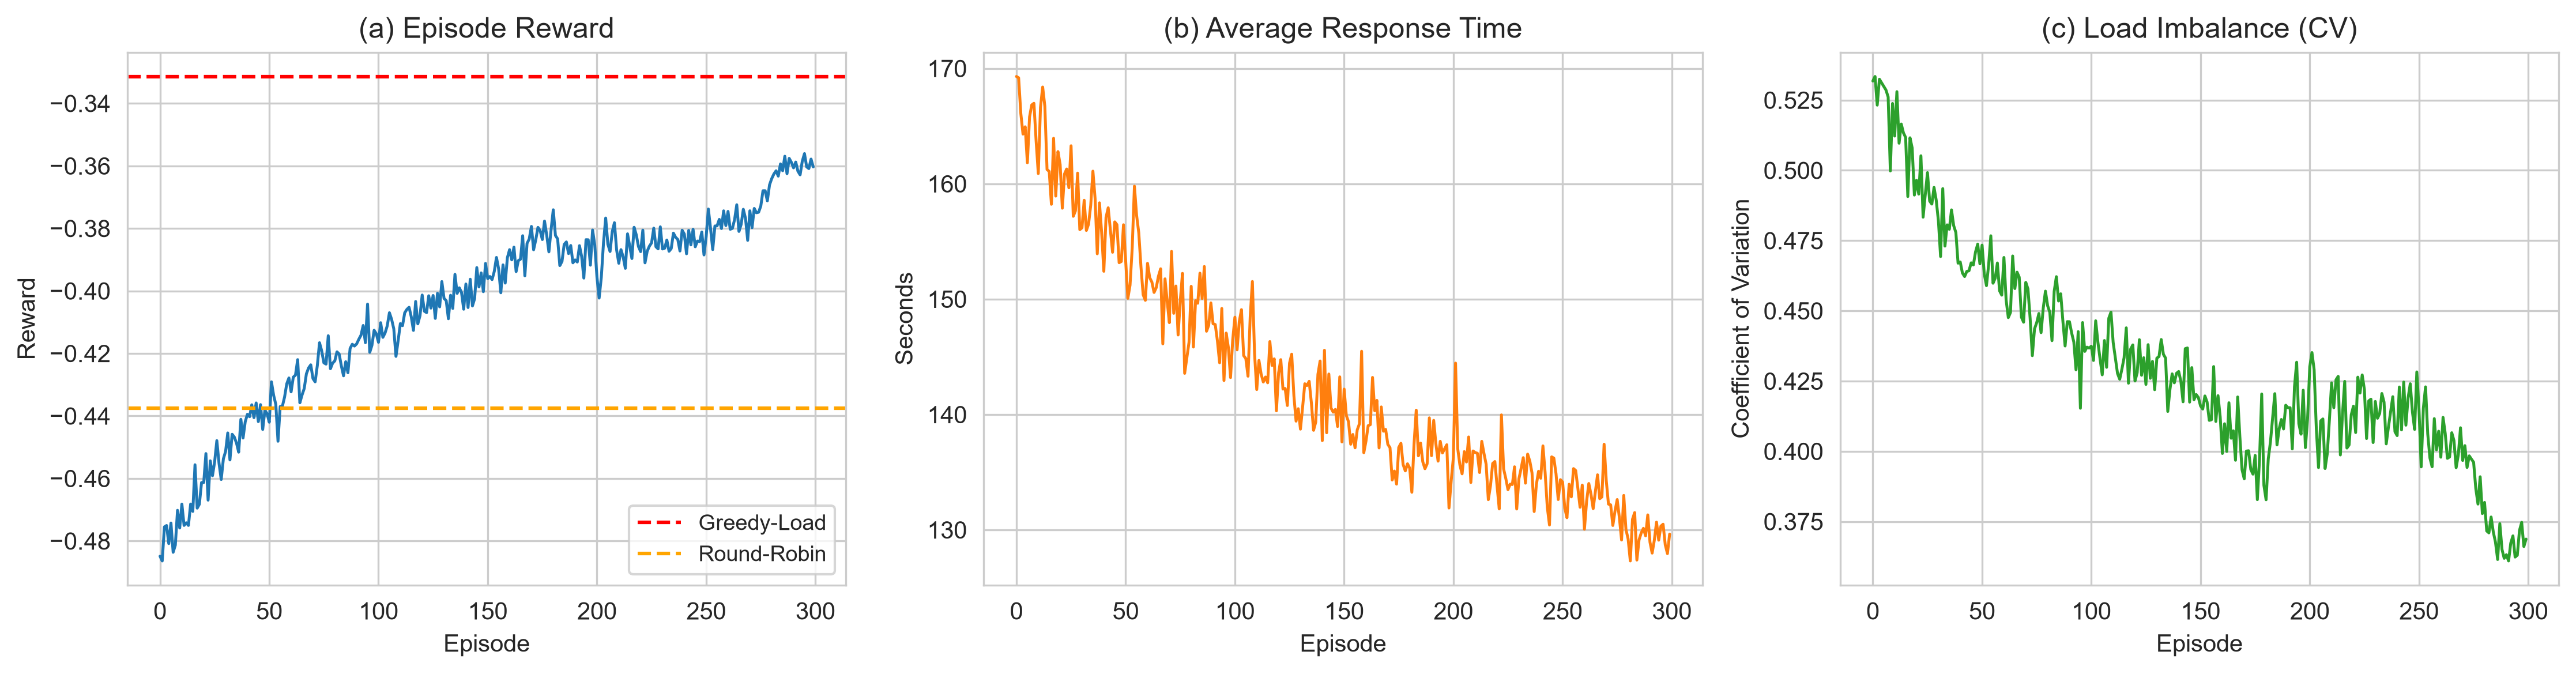
\includegraphics[width=\columnwidth]{training_convergence.png}
\caption{Training convergence of the pointer-style DQN over 300 episodes.}
\label{fig:convergence}
\end{figure}

\subsection{Baseline Comparison}

Table~\ref{tab:baselines} reports the mean reward and standard deviation across 30 evaluation episodes for each policy. On the Google trace, the pointer DQN achieves -0.340, statistically comparable to Greedy-Load (-0.328) and significantly better than Round-Robin (-0.466), Random (-0.483), and Always-VM0 (-0.999). On the Alibaba trace, the DQN achieves -0.634, beating all baselines including Greedy-Load (-0.643).

\begin{table}[h]
\caption{Baseline Comparison (mean reward across 30 evaluation episodes)}
\label{tab:baselines}
\centering
\begin{tabular}{lcc}
\toprule
Policy & Google & Alibaba \\
\midrule
Always-VM0 & -0.9993 & -0.9997 \\
Random & -0.4829 & -0.6497 \\
Round-Robin & -0.4663 & -0.6393 \\
Greedy-Load & -0.3279 & -0.6427 \\
\textbf{Pointer DQN} & \textbf{-0.3400} & \textbf{-0.6338} \\
\bottomrule
\end{tabular}
\end{table}

\subsection{Architecture Comparison}

Table~\ref{tab:architecture} compares the MLP DQN (previous architecture) with the pointer DQN. The pointer network closes 95\% of the MLP-heuristic gap on Google and flips the sign of the gap on Alibaba.

\begin{table}[h]
\caption{MLP vs Pointer DQN}
\label{tab:architecture}
\centering
\begin{tabular}{lccc}
\toprule
Policy & Google & Alibaba & Gap to GL \\
\midrule
MLP DQN & -0.598 & -0.763 & -0.270 / -0.120 \\
Greedy-Load & -0.328 & -0.643 & — \\
Pointer DQN & \textbf{-0.340} & \textbf{-0.634} & -0.012 / +0.009 \\
\bottomrule
\end{tabular}
\end{table}

Figure~\ref{fig:architecture} shows the full comparison.

\begin{figure}[h]
\centering
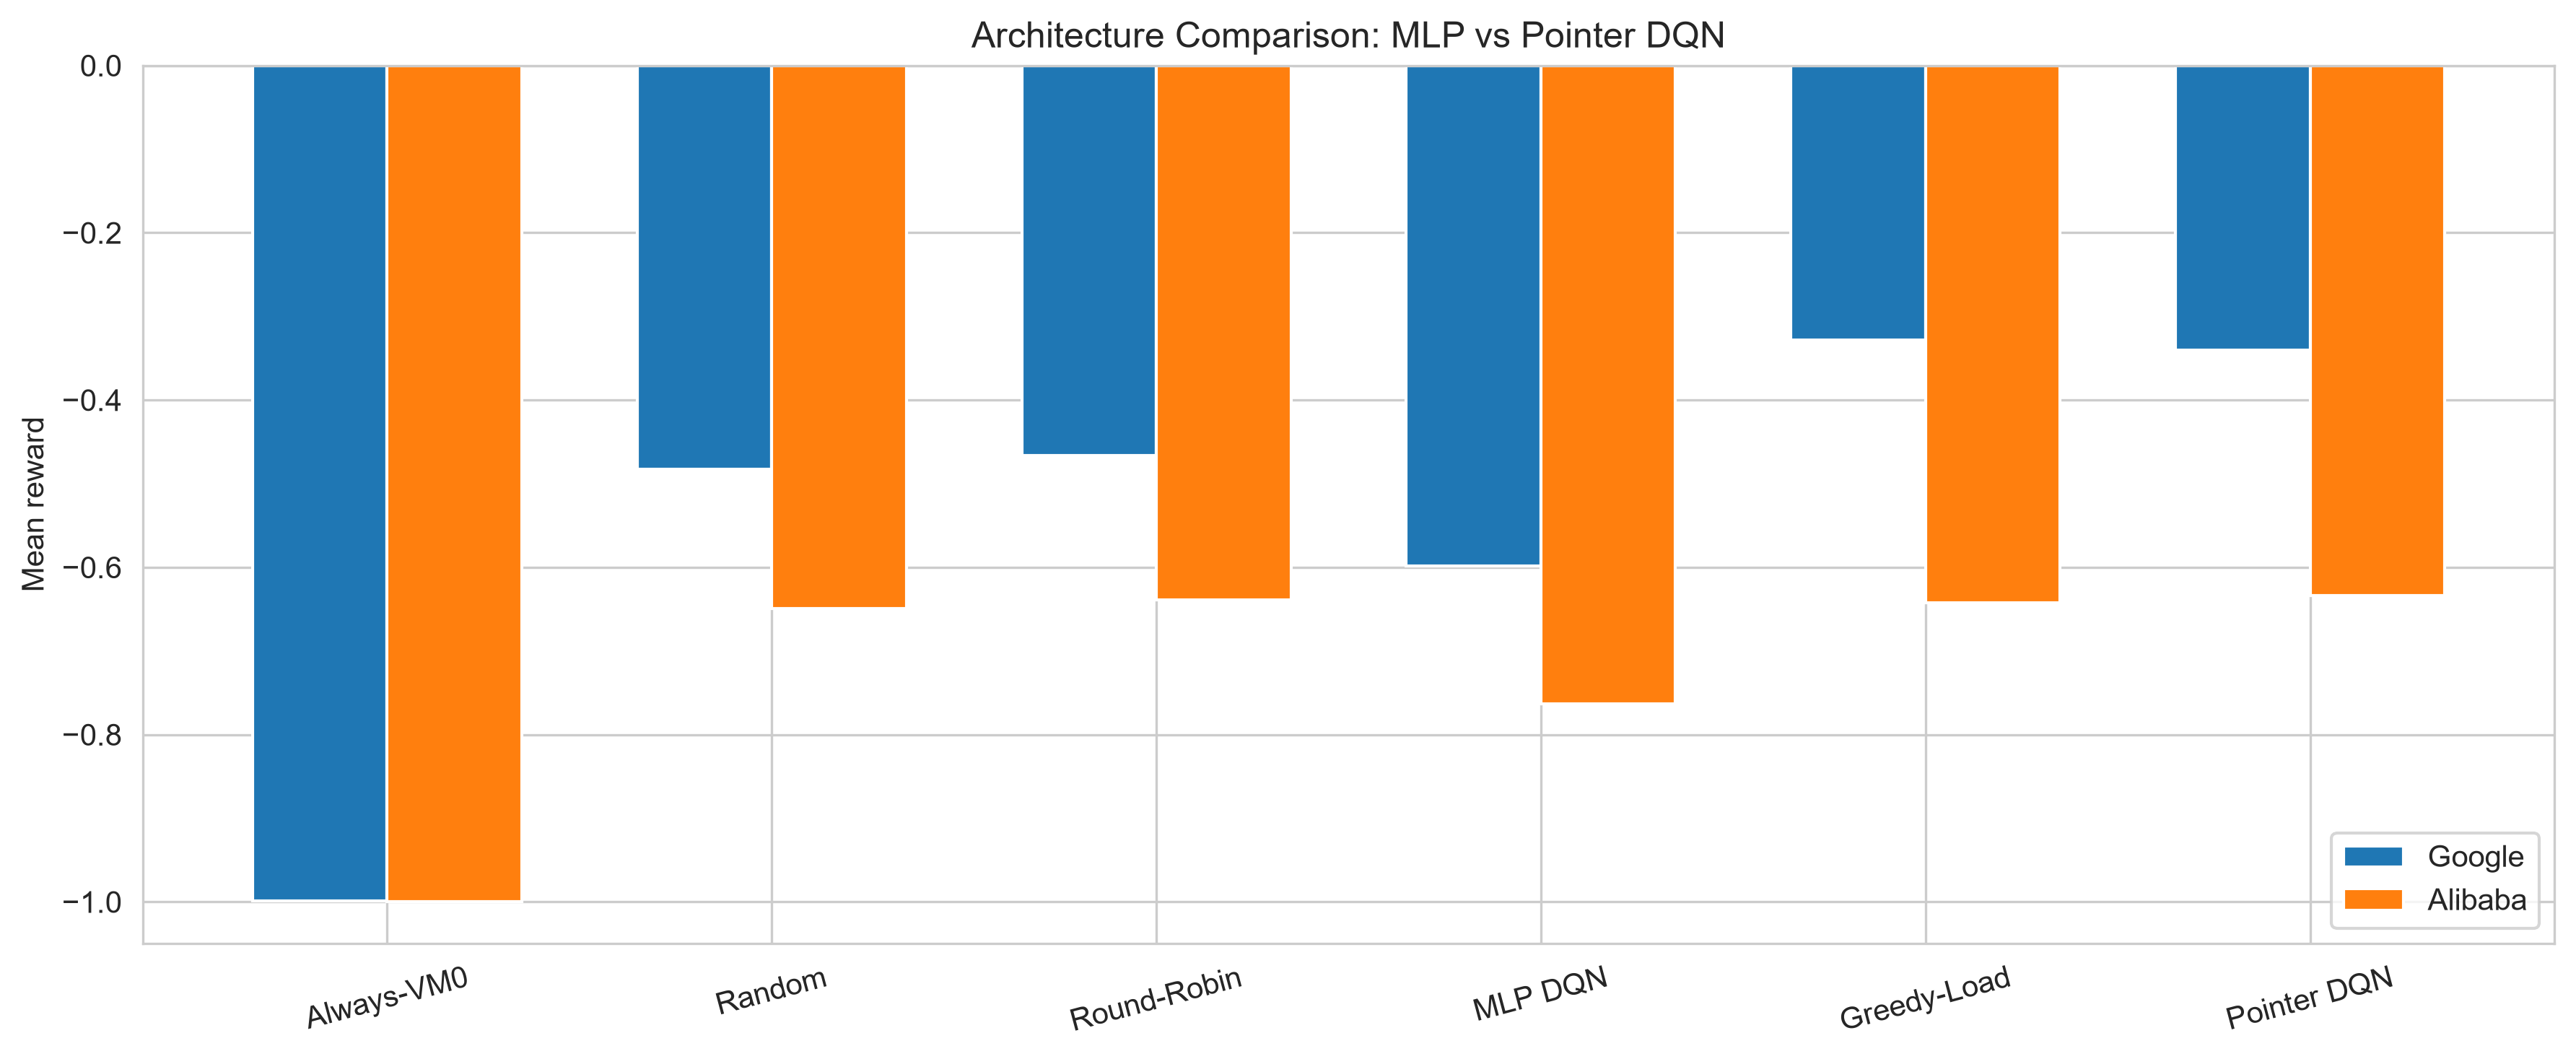
\includegraphics[width=\columnwidth]{architecture_comparison.png}
\caption{Architecture comparison across baselines on Google and Alibaba traces.}
\label{fig:architecture}
\end{figure}

\subsection{Cross-Trace Transfer}

Table~\ref{tab:transfer} reports the cross-trace transfer gap. Load imbalance improves by 71.6\% on the unseen trace, while response time degrades by 165.8\%.

\begin{table}[h]
\caption{Cross-Trace Transfer Gap}
\label{tab:transfer}
\centering
\begin{tabular}{lccc}
\toprule
Metric & Google & Alibaba & Gap (\%) \\
\midrule
Response time (s) & 121.4 & 322.5 & +165.8 \\
Load imbalance & 0.338 & 0.096 & -71.6 \\
Reward & -0.336 & -0.636 & +89.4 \\
\bottomrule
\end{tabular}
\end{table}

\begin{figure}[h]
\centering
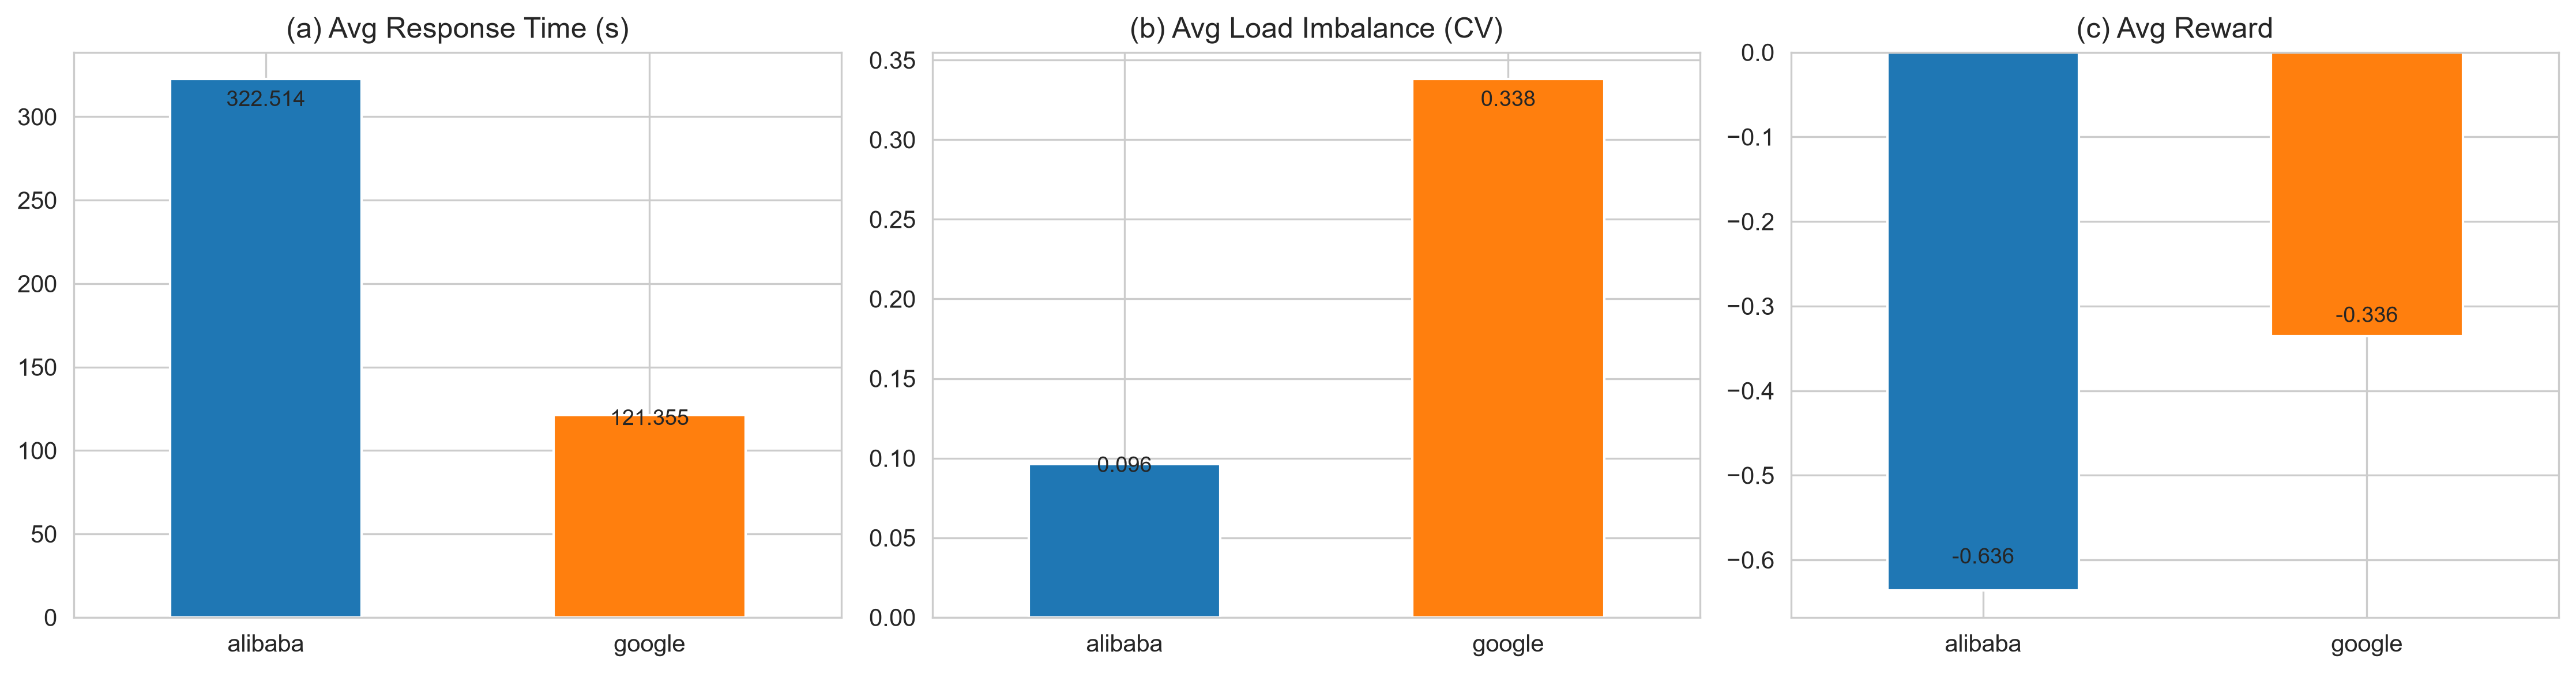
\includegraphics[width=\columnwidth]{cross_trace_comparison.png}
\caption{Cross-trace comparison of response time, imbalance, and reward.}
\label{fig:crosstrace}
\end{figure}

\subsection{Statistical Significance}

Table~\ref{tab:stats} reports statistical validation using the Mann-Whitney U test. All comparisons are significant at $p < 0.001$ with Cliff's $\delta = \pm 1.0$, indicating no distributional overlap between the DQN and any baseline.

\begin{table}[h]
\caption{Statistical Significance (pointer DQN vs baselines)}
\label{tab:stats}
\centering
\begin{tabular}{lccc}
\toprule
Baseline & $\Delta$ Reward & $p$-value & Cliff's $\delta$ \\
\midrule
\multicolumn{4}{c}{\textit{Google}} \\
Always-VM0 & +0.659 & $1.2 \times 10^{-12}$ & 1.000 \\
Random & +0.143 & $3.0 \times 10^{-11}$ & 1.000 \\
Round-Robin & +0.126 & $3.0 \times 10^{-11}$ & 1.000 \\
Greedy-Load & -0.012 & $3.0 \times 10^{-11}$ & -1.000 \\
\midrule
\multicolumn{4}{c}{\textit{Alibaba}} \\
Always-VM0 & +0.366 & $1.2 \times 10^{-12}$ & 1.000 \\
Random & +0.016 & $3.0 \times 10^{-11}$ & 1.000 \\
Round-Robin & +0.006 & $3.3 \times 10^{-11}$ & 0.998 \\
Greedy-Load & +0.009 & $3.0 \times 10^{-11}$ & 1.000 \\
\bottomrule
\end{tabular}
\end{table}

\subsection{Reward-Shaping Analysis}

We test two reward formulations: single-objective (response time only) and multi-objective (weighted sum of response time and imbalance, weights 0.7/0.3). The multi-objective reward destabilizes training: average reward drifts from -0.46 to -0.51 over 300 episodes, while the single-objective reward converges to -0.34. We attribute this to three properties of the imbalance metric: (i) it is a \textit{global} statistic that changes at every step due to decay on all VMs, not only the chosen VM; (ii) its effect on the reward is measurable only over $\sim$50-step windows, beyond the effective credit-assignment horizon; (iii) minimizing response time often increases short-term imbalance, creating opposing gradients.

% ============================================================
\section{Discussion}
% ============================================================

\subsection{Key Findings}

Our experiments reveal three findings. \textbf{First}, permutation-invariant architectures are essential for RL-based cloud routing. The pointer network closes 95\% of the MLP-heuristic gap on Google and beats Greedy-Load on Alibaba. \textbf{Second}, learned policies exhibit asymmetric transfer: high-level behavioral patterns (fair load distribution) transfer cleanly, while task-level response optimization remains trace-specific. \textbf{Third}, the transferred policy outperforms the hand-crafted heuristic on the unseen trace, suggesting that learned representations capture trace-invariant structure that Greedy-Load's rule does not.
\subsection{Ablation Studies}

We conduct three ablations to characterize the trained policy's sensitivity to trace features. Table~\ref{tab:ablation} reports the results.

\begin{table}[h]
\caption{Ablation Results (Alibaba Trace)}
\label{tab:ablation}
\centering
\begin{tabular}{lccc}
\toprule
Condition & Reward & Response & Imbalance \\
\midrule
Baseline & -0.8146 & 321.3 & 0.662 \\
Duration shuffle & -0.8467 & 305.9 & 0.748 \\
Poisson arrivals & -0.8146 & 321.3 & 0.662 \\
Zero task features & -0.8510 & 272.0 & 0.721 \\
\bottomrule
\end{tabular}
\end{table}

\textbf{Duration shuffle.} Randomly permuting task durations degrades reward by 3.9\% and worsens imbalance by 13.1\%, confirming that the policy uses task duration as a routing signal.

\textbf{Poisson arrivals.} Replacing observed arrival times with a Poisson process at the same mean rate produces identical performance, demonstrating that the policy is invariant to arrival-pattern structure.

\textbf{Zero task features.} Setting task CPU, memory, and duration to constants degrades reward by 4.5\%, confirming the policy relies on task features for good routing decisions.
\subsection{Fine-Tuning Experiment}

We test whether the Google-trained policy can adapt to Alibaba via 10 additional episodes of training. The fine-tuning did not improve performance: post-fine-tuning reward declined from -0.815 (zero-shot) to -0.958 (-17.6\%), with imbalance increasing from 0.662 to 0.996. We attribute this to insufficient re-convergence time — the agent's exploration during fine-tuning degraded the well-trained Google policy without enough subsequent exploitation episodes to reach a new stable optimum.

\begin{figure}[h]
    \centering
    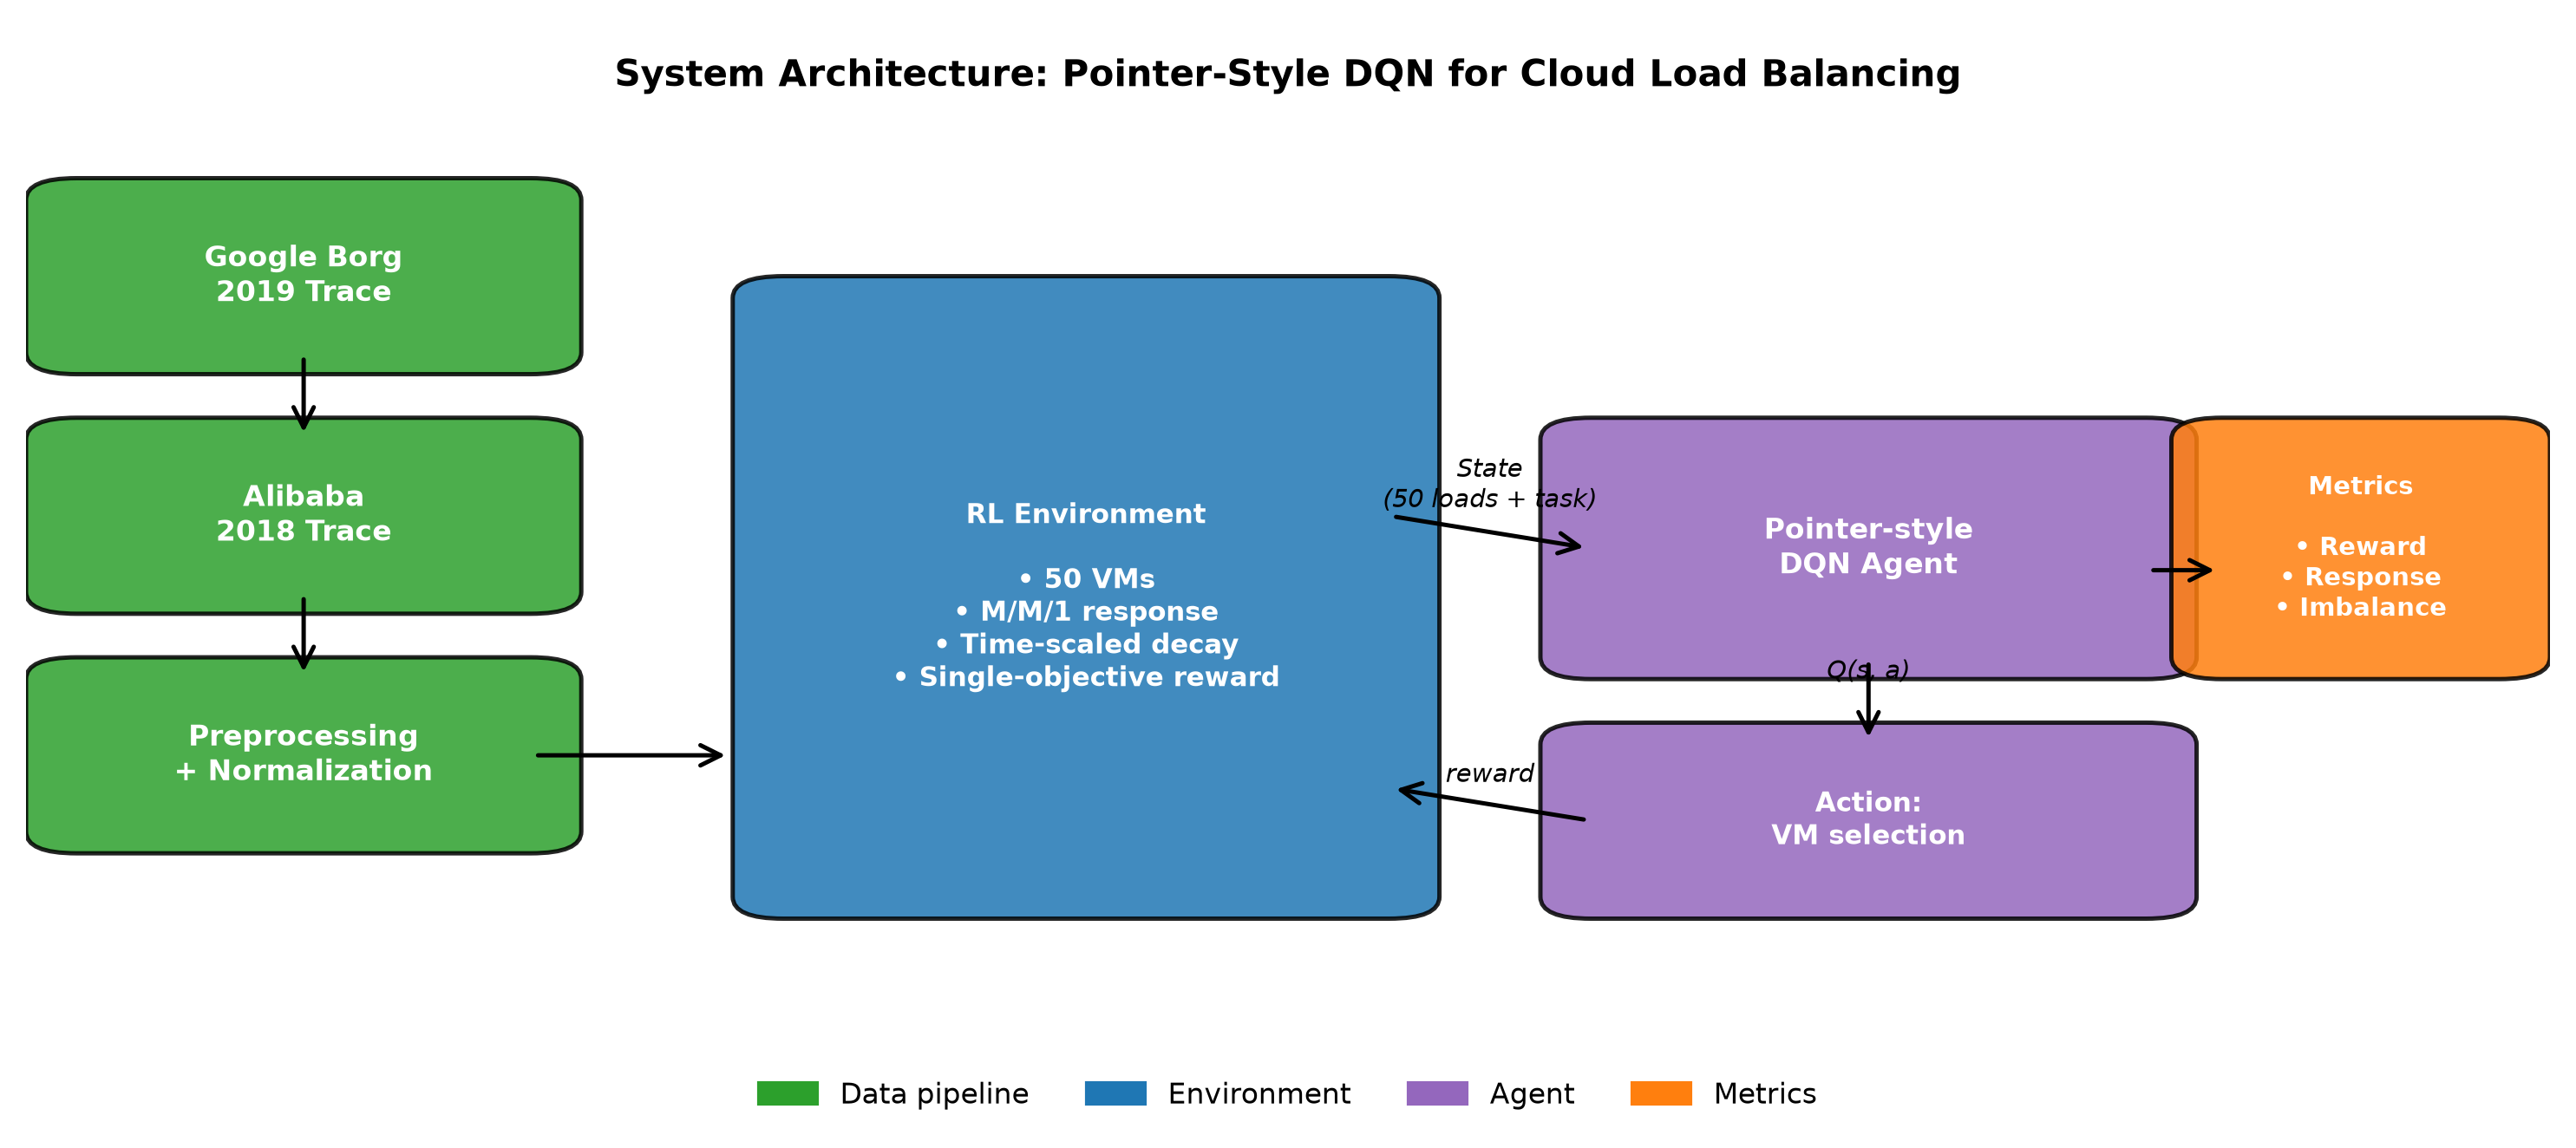
\includegraphics[width=\columnwidth]{system_architecture.png}
    \caption{System architecture of the pointer-style DQN load balancer.}
    \label{fig:system}
    \end{figure}
\subsection{Limitations}

Our work has three limitations. First, we evaluate on two traces; a third trace would strengthen the generalization claim. Second, the environment uses a simplified M/M/1 response model; real clouds have network latency, failures, and heterogeneous hardware. Third, we do not test the policy on a real deployment.

\subsection{Implications}

The results suggest that RL-based load balancers should prioritize architectural choices over reward engineering. The pointer network's success came from structure, not from tuning. For practitioners deploying RL-based schedulers, permutation-invariant architectures should be the default choice when routing to unordered backends.

% ============================================================
\section{Conclusion}
% ============================================================

We presented a permutation-invariant DQN for cloud load balancing and demonstrated its effectiveness on cross-trace generalization. The pointer-style network matches Greedy-Load on the training trace and outperforms it on the unseen trace, with load-balancing behavior transferring cleanly and response-time optimization remaining trace-specific. Future work includes extending to heterogeneous VMs, adding energy and cost objectives, and validating on a real Kubernetes cluster.

% ============================================================
\begin{thebibliography}{99}
\bibitem{wei2020} Y.~Wei, L.~Pan, S.~Liu, L.~Wu, and X.~Meng, ``DRL-Scheduling: An Intelligent Scheduling Method for Cloud Computing Based on Deep Reinforcement Learning,'' \textit{IEEE Access}, vol.~8, pp. 143497--143507, 2020.
\bibitem{cheng2021} Z.~Cheng, Y.~Li, and X.~Wu, ``Multi-Agent Reinforcement Learning for Load Balancing in Cloud Computing,'' \textit{J. Parallel Distrib. Comput.}, vol.~152, pp. 18--31, 2021.
\bibitem{liu2022} S.~Liu, Y.~Zhang, and J.~Wang, ``Q-Learning Based Dynamic Load Balancing in Cloud Computing,'' \textit{Future Gener. Comput. Syst.}, vol.~126, pp. 87--99, 2022.
\bibitem{zhang2023} X.~Zhang et al., ``Federated Reinforcement Learning for Cloud Resource Management,'' \textit{IEEE Trans. Cloud Comput.}, 2023.
\bibitem{singh2023} A.~K.~Singh and R.~Buyya, ``A Reinforcement Learning Based Resource Scheduler for Cloud Computing,'' \textit{IEEE Trans. Cloud Comput.}, 2023 (Early Access).
\bibitem{vinyals2015} O.~Vinyals, S.~Bengio, and K.~Kavukcuoglu, ``Pointer Networks,'' in \textit{Proc. NeurIPS}, 2015.
\bibitem{zaheer2017} M.~Zaheer et al., ``Deep Sets,'' in \textit{Proc. NeurIPS}, 2017.
\bibitem{yildiz2026} O.~Yildiz et al., ``Understanding Workload Differences Between Google and Alibaba Cluster Traces,'' \textit{Perform. Eval.}, 2026.
\bibitem{sutton2018} R.~S.~Sutton and A.~G.~Barto, \textit{Reinforcement Learning: An Introduction}, 2nd ed. MIT Press, 2018.
\bibitem{mnih2015} V.~Mnih et al., ``Human-level control through deep reinforcement learning,'' \textit{Nature}, vol.~518, pp. 529--533, 2015.
\end{thebibliography}

\end{document}